\documentclass[a4paper]{scrartcl}

\usepackage[utf8]{inputenc}
\usepackage[T1]{fontenc}
\usepackage{lmodern}
\usepackage[naustrian]{babel}
\usepackage{amsmath}
\usepackage{verbatim}
\usepackage{scrpage2}
\usepackage[dvipsnames]{xcolor}
\usepackage{titling}
\usepackage{a4wide}
\usepackage{pdfpages}
\usepackage{tikz}
\usepackage{titling}
\usepackage{float}
\usepackage{graphicx}
\usepackage{hyperref}

\pagestyle{scrheadings}
\clearscrheadfoot

\title{WatchPLB Hardware}
\author{Samuel Hick}
\date{19.06.2018}

%% scource-code listings
\usepackage{listingsutf8, scrhack}
\usepackage{courier}
\lstset{%
    basicstyle=\footnotesize\ttfamily,
    breaklines=true,
    commentstyle=\color{OliveGreen},
    keywordstyle=\color{MidnightBlue},
    stringstyle=\color{Maroon},
    escapeinside={\%*}{*)},
    inputencoding=utf8/latin1,
    frame=single,
    numbers=left,
    stepnumber=1
}




\begin{document}
\listoffigures   

\newpage

\begin{figure}[htb]\centering
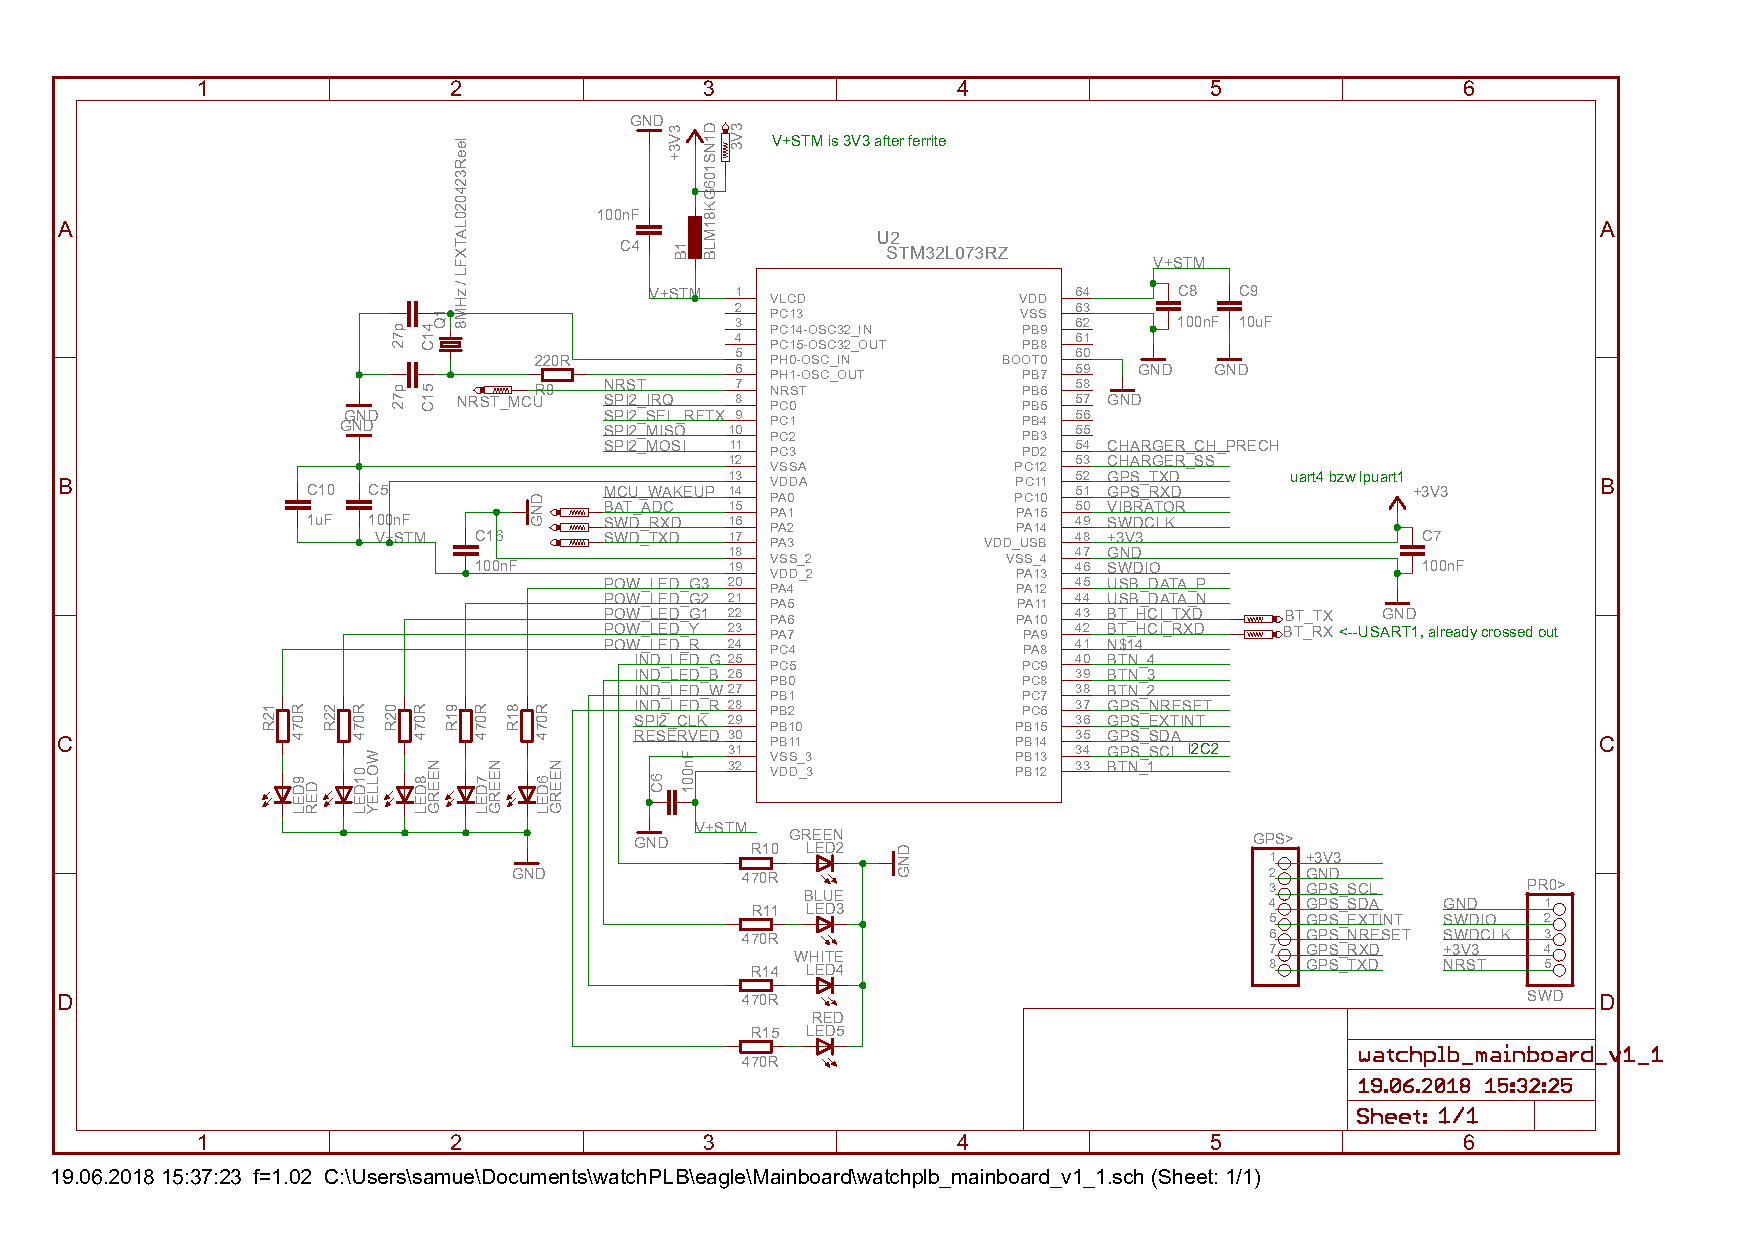
\includegraphics[page=1, angle=90, width=\linewidth]{../Mainboard/watchplb_mainboard_v1_1.pdf}
\caption{Mikrocontroller STM32F0}
\label{fig:abb1}
\end{figure}

\begin{figure}[htb]\centering
\includegraphics[page=2, angle=90, width=\linewidth]{../Mainboard/watchplb_mainboard_v1_1.pdf}
\caption{USB-To-UART und USB des STM}
\label{fig:abb1}
\end{figure}

\begin{figure}[htb]\centering
\includegraphics[page=3, angle=90, width=\linewidth]{../Mainboard/watchplb_mainboard_v1_1.pdf}
\caption{Bluetooth-Modul}
\label{fig:abb1}
\end{figure}

\begin{figure}[htb]\centering
\includegraphics[page=5, angle=90, width=\linewidth]{../Mainboard/watchplb_mainboard_v1_1.pdf}
\caption{Lithium-Ionen-Akku Schutzschaltung}
\label{fig:abb1}
\end{figure}

\begin{figure}[htb]\centering
\includegraphics[page=6, angle=90, width=\linewidth]{../Mainboard/watchplb_mainboard_v1_1.pdf}
\caption{Akkuladeschaltung und Spannungsregler}
\label{fig:abb1}
\end{figure}

\begin{figure}[htb]\centering
\includegraphics[page=7, angle=90, width=\linewidth]{../Mainboard/watchplb_mainboard_v1_1.pdf}
\caption{Taster, WakeUp, Vibrationsmotor}
\label{fig:abb1}
\end{figure}

\begin{figure}[htb]\centering
\includegraphics[page=8, angle=90, width=\linewidth]{../Mainboard/watchplb_mainboard_v1_1.pdf}
\caption{Funk}
\label{fig:abb1}
\end{figure}

\begin{figure}[htb]\centering
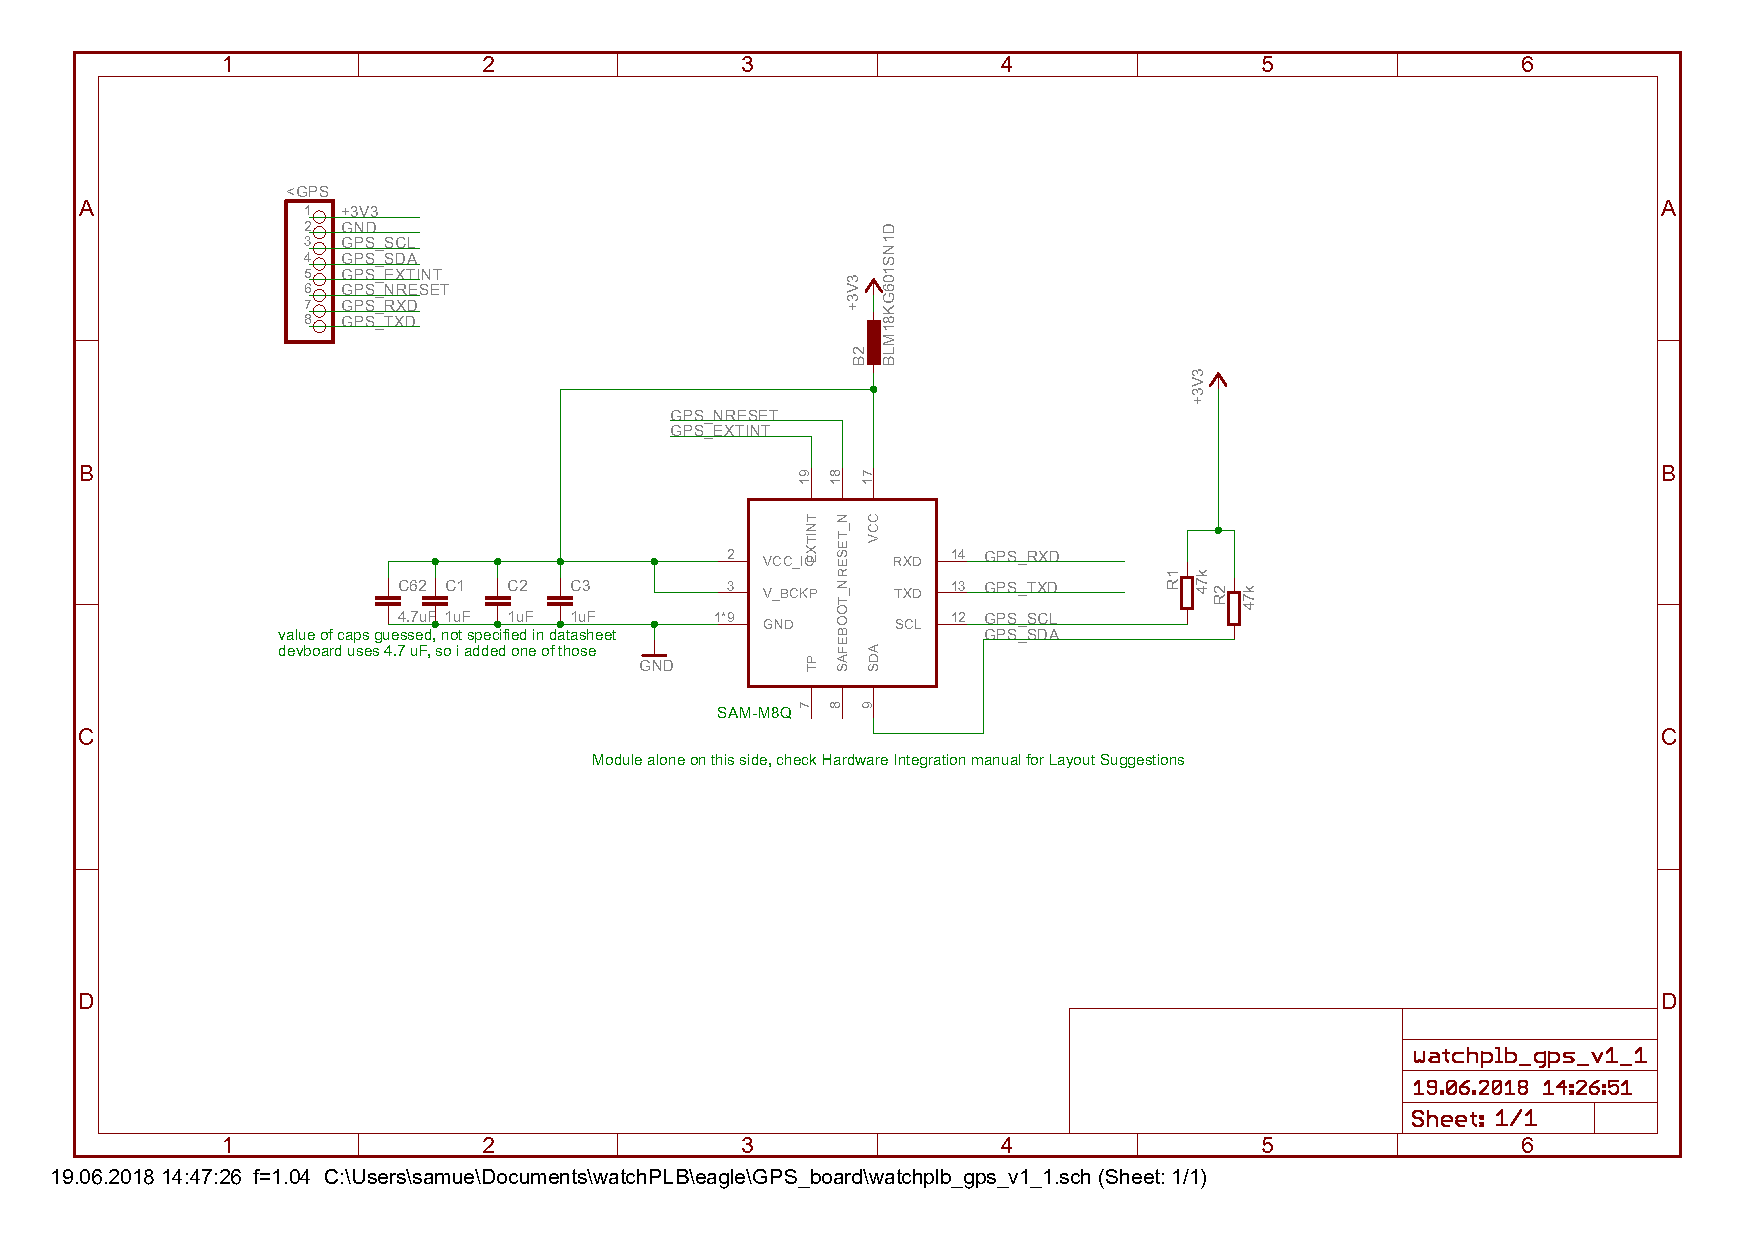
\includegraphics[page=1, angle=90, width=\linewidth]{../GPS_board/watchplb_gps_v1_1.pdf}
\caption{GPS-Modul}
\label{fig:abb1}
\end{figure}



\end{document}